\documentclass[dvipdfmx]{standalone}
% \documentclass[b5paper,papersize,dvipdfmx]{jsarticle}
% \documentclass[b5paper,papersize,dvipdfmx]{jsbook}
%
\usepackage{amsmath}
\usepackage{physics}
\usepackage{here}
\usepackage[dvipdfmx]{graphicx}
% 必須
\usepackage{gnuplot-lua-tikz}
\usepackage{tikz}

\begin{document}
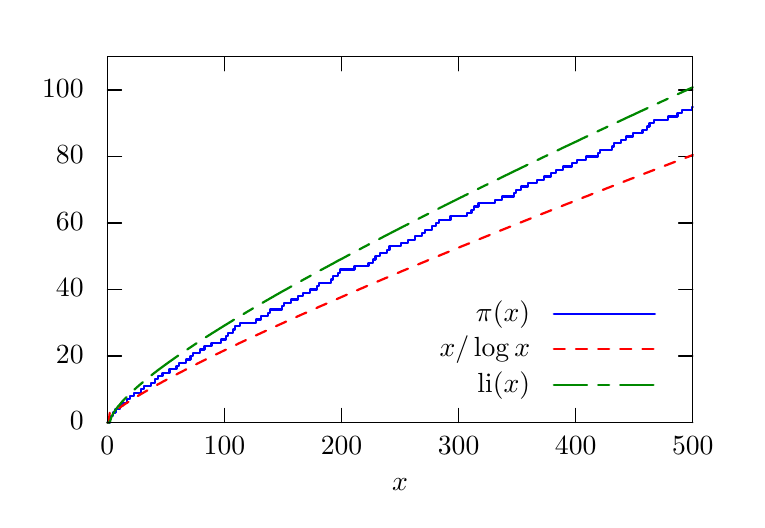
\begin{tikzpicture}[gnuplot]
%% generated with GNUPLOT 5.1p0 (Lua 5.3; terminal rev. 99, script rev. 100)
%% 木 11/22 15:28:55 2018
\path (0.000,0.000) rectangle (9.000,6.000);
\gpcolor{color=gp lt color border}
\gpsetlinetype{gp lt border}
\gpsetdashtype{gp dt solid}
\gpsetlinewidth{1.00}
\draw[gp path] (1.012,0.985)--(1.192,0.985);
\draw[gp path] (8.447,0.985)--(8.267,0.985);
\node[gp node right] at (0.828,0.985) {$0$};
\draw[gp path] (1.012,1.830)--(1.192,1.830);
\draw[gp path] (8.447,1.830)--(8.267,1.830);
\node[gp node right] at (0.828,1.830) {$20$};
\draw[gp path] (1.012,2.674)--(1.192,2.674);
\draw[gp path] (8.447,2.674)--(8.267,2.674);
\node[gp node right] at (0.828,2.674) {$40$};
\draw[gp path] (1.012,3.519)--(1.192,3.519);
\draw[gp path] (8.447,3.519)--(8.267,3.519);
\node[gp node right] at (0.828,3.519) {$60$};
\draw[gp path] (1.012,4.364)--(1.192,4.364);
\draw[gp path] (8.447,4.364)--(8.267,4.364);
\node[gp node right] at (0.828,4.364) {$80$};
\draw[gp path] (1.012,5.209)--(1.192,5.209);
\draw[gp path] (8.447,5.209)--(8.267,5.209);
\node[gp node right] at (0.828,5.209) {$100$};
\draw[gp path] (1.012,0.985)--(1.012,1.165);
\draw[gp path] (1.012,5.631)--(1.012,5.451);
\node[gp node center] at (1.012,0.677) {$0$};
\draw[gp path] (2.499,0.985)--(2.499,1.165);
\draw[gp path] (2.499,5.631)--(2.499,5.451);
\node[gp node center] at (2.499,0.677) {$100$};
\draw[gp path] (3.986,0.985)--(3.986,1.165);
\draw[gp path] (3.986,5.631)--(3.986,5.451);
\node[gp node center] at (3.986,0.677) {$200$};
\draw[gp path] (5.473,0.985)--(5.473,1.165);
\draw[gp path] (5.473,5.631)--(5.473,5.451);
\node[gp node center] at (5.473,0.677) {$300$};
\draw[gp path] (6.960,0.985)--(6.960,1.165);
\draw[gp path] (6.960,5.631)--(6.960,5.451);
\node[gp node center] at (6.960,0.677) {$400$};
\draw[gp path] (8.447,0.985)--(8.447,1.165);
\draw[gp path] (8.447,5.631)--(8.447,5.451);
\node[gp node center] at (8.447,0.677) {$500$};
\draw[gp path] (1.012,5.631)--(1.012,0.985)--(8.447,0.985)--(8.447,5.631)--cycle;
\node[gp node center] at (4.729,0.215) {$x$};
\node[gp node right] at (6.498,2.365) {$\pi(x)$};
\gpcolor{rgb color={0.000,0.000,1.000}}
\gpsetlinewidth{2.00}
\draw[gp path] (6.682,2.365)--(7.966,2.365);
\draw[gp path] (1.012,0.985)--(1.027,0.985)--(1.042,0.985)--(1.042,1.027)--(1.057,1.027)%
  --(1.057,1.069)--(1.071,1.069)--(1.086,1.069)--(1.086,1.112)--(1.101,1.112)--(1.116,1.112)%
  --(1.116,1.154)--(1.131,1.154)--(1.146,1.154)--(1.161,1.154)--(1.176,1.154)--(1.176,1.196)%
  --(1.190,1.196)--(1.205,1.196)--(1.205,1.238)--(1.220,1.238)--(1.235,1.238)--(1.250,1.238)%
  --(1.265,1.238)--(1.265,1.281)--(1.280,1.281)--(1.295,1.281)--(1.295,1.323)--(1.309,1.323)%
  --(1.324,1.323)--(1.339,1.323)--(1.354,1.323)--(1.354,1.365)--(1.369,1.365)--(1.384,1.365)%
  --(1.399,1.365)--(1.413,1.365)--(1.428,1.365)--(1.443,1.365)--(1.443,1.407)--(1.458,1.407)%
  --(1.473,1.407)--(1.473,1.450)--(1.488,1.450)--(1.503,1.450)--(1.518,1.450)--(1.532,1.450)%
  --(1.547,1.450)--(1.562,1.450)--(1.562,1.492)--(1.577,1.492)--(1.592,1.492)--(1.607,1.492)%
  --(1.622,1.492)--(1.622,1.534)--(1.637,1.534)--(1.651,1.534)--(1.651,1.576)--(1.666,1.576)%
  --(1.681,1.576)--(1.696,1.576)--(1.711,1.576)--(1.711,1.619)--(1.726,1.619)--(1.741,1.619)%
  --(1.756,1.619)--(1.770,1.619)--(1.785,1.619)--(1.800,1.619)--(1.800,1.661)--(1.815,1.661)%
  --(1.830,1.661)--(1.845,1.661)--(1.860,1.661)--(1.874,1.661)--(1.889,1.661)--(1.889,1.703)%
  --(1.904,1.703)--(1.919,1.703)--(1.919,1.745)--(1.934,1.745)--(1.949,1.745)--(1.964,1.745)%
  --(1.979,1.745)--(1.993,1.745)--(2.008,1.745)--(2.008,1.787)--(2.023,1.787)--(2.038,1.787)%
  --(2.053,1.787)--(2.068,1.787)--(2.068,1.830)--(2.083,1.830)--(2.098,1.830)--(2.098,1.872)%
  --(2.112,1.872)--(2.127,1.872)--(2.142,1.872)--(2.157,1.872)--(2.172,1.872)--(2.187,1.872)%
  --(2.187,1.914)--(2.202,1.914)--(2.216,1.914)--(2.231,1.914)--(2.246,1.914)--(2.246,1.956)%
  --(2.261,1.956)--(2.276,1.956)--(2.291,1.956)--(2.306,1.956)--(2.321,1.956)--(2.335,1.956)%
  --(2.335,1.999)--(2.350,1.999)--(2.365,1.999)--(2.380,1.999)--(2.395,1.999)--(2.410,1.999)%
  --(2.425,1.999)--(2.440,1.999)--(2.454,1.999)--(2.454,2.041)--(2.469,2.041)--(2.484,2.041)%
  --(2.499,2.041)--(2.514,2.041)--(2.514,2.083)--(2.529,2.083)--(2.544,2.083)--(2.544,2.125)%
  --(2.558,2.125)--(2.573,2.125)--(2.588,2.125)--(2.603,2.125)--(2.603,2.168)--(2.618,2.168)%
  --(2.633,2.168)--(2.633,2.210)--(2.648,2.210)--(2.663,2.210)--(2.677,2.210)--(2.692,2.210)%
  --(2.692,2.252)--(2.707,2.252)--(2.722,2.252)--(2.737,2.252)--(2.752,2.252)--(2.767,2.252)%
  --(2.782,2.252)--(2.796,2.252)--(2.811,2.252)--(2.826,2.252)--(2.841,2.252)--(2.856,2.252)%
  --(2.871,2.252)--(2.886,2.252)--(2.900,2.252)--(2.900,2.294)--(2.915,2.294)--(2.930,2.294)%
  --(2.945,2.294)--(2.960,2.294)--(2.960,2.337)--(2.975,2.337)--(2.990,2.337)--(3.005,2.337)%
  --(3.019,2.337)--(3.034,2.337)--(3.049,2.337)--(3.049,2.379)--(3.064,2.379)--(3.079,2.379)%
  --(3.079,2.421)--(3.094,2.421)--(3.109,2.421)--(3.124,2.421)--(3.138,2.421)--(3.153,2.421)%
  --(3.168,2.421)--(3.183,2.421)--(3.198,2.421)--(3.213,2.421)--(3.228,2.421)--(3.228,2.463)%
  --(3.243,2.463)--(3.257,2.463)--(3.257,2.506)--(3.272,2.506)--(3.287,2.506)--(3.302,2.506)%
  --(3.317,2.506)--(3.332,2.506)--(3.347,2.506)--(3.347,2.548)--(3.361,2.548)--(3.376,2.548)%
  --(3.391,2.548)--(3.406,2.548)--(3.421,2.548)--(3.436,2.548)--(3.436,2.590)--(3.451,2.590)%
  --(3.466,2.590)--(3.480,2.590)--(3.495,2.590)--(3.495,2.632)--(3.510,2.632)--(3.525,2.632)%
  --(3.540,2.632)--(3.555,2.632)--(3.570,2.632)--(3.585,2.632)--(3.585,2.674)--(3.599,2.674)%
  --(3.614,2.674)--(3.629,2.674)--(3.644,2.674)--(3.659,2.674)--(3.674,2.674)--(3.674,2.717)%
  --(3.689,2.717)--(3.703,2.717)--(3.703,2.759)--(3.718,2.759)--(3.733,2.759)--(3.748,2.759)%
  --(3.763,2.759)--(3.778,2.759)--(3.793,2.759)--(3.808,2.759)--(3.822,2.759)--(3.837,2.759)%
  --(3.852,2.759)--(3.852,2.801)--(3.867,2.801)--(3.882,2.801)--(3.882,2.843)--(3.897,2.843)%
  --(3.912,2.843)--(3.927,2.843)--(3.941,2.843)--(3.941,2.886)--(3.956,2.886)--(3.971,2.886)%
  --(3.971,2.928)--(3.986,2.928)--(4.001,2.928)--(4.016,2.928)--(4.031,2.928)--(4.045,2.928)%
  --(4.060,2.928)--(4.075,2.928)--(4.090,2.928)--(4.105,2.928)--(4.120,2.928)--(4.135,2.928)%
  --(4.150,2.928)--(4.150,2.970)--(4.164,2.970)--(4.179,2.970)--(4.194,2.970)--(4.209,2.970)%
  --(4.224,2.970)--(4.239,2.970)--(4.254,2.970)--(4.269,2.970)--(4.283,2.970)--(4.298,2.970)%
  --(4.313,2.970)--(4.328,2.970)--(4.328,3.012)--(4.343,3.012)--(4.358,3.012)--(4.373,3.012)%
  --(4.387,3.012)--(4.387,3.055)--(4.402,3.055)--(4.417,3.055)--(4.417,3.097)--(4.432,3.097)%
  --(4.447,3.097)--(4.462,3.097)--(4.477,3.097)--(4.477,3.139)--(4.492,3.139)--(4.506,3.139)%
  --(4.521,3.139)--(4.536,3.139)--(4.551,3.139)--(4.566,3.139)--(4.566,3.181)--(4.581,3.181)%
  --(4.596,3.181)--(4.596,3.224)--(4.611,3.224)--(4.625,3.224)--(4.640,3.224)--(4.655,3.224)%
  --(4.670,3.224)--(4.685,3.224)--(4.700,3.224)--(4.715,3.224)--(4.730,3.224)--(4.744,3.224)%
  --(4.744,3.266)--(4.759,3.266)--(4.774,3.266)--(4.789,3.266)--(4.804,3.266)--(4.819,3.266)%
  --(4.834,3.266)--(4.834,3.308)--(4.848,3.308)--(4.863,3.308)--(4.878,3.308)--(4.893,3.308)%
  --(4.908,3.308)--(4.923,3.308)--(4.923,3.350)--(4.938,3.350)--(4.953,3.350)--(4.967,3.350)%
  --(4.982,3.350)--(4.997,3.350)--(5.012,3.350)--(5.012,3.392)--(5.027,3.392)--(5.042,3.392)%
  --(5.042,3.435)--(5.057,3.435)--(5.072,3.435)--(5.086,3.435)--(5.101,3.435)--(5.116,3.435)%
  --(5.131,3.435)--(5.131,3.477)--(5.146,3.477)--(5.161,3.477)--(5.176,3.477)--(5.190,3.477)%
  --(5.190,3.519)--(5.205,3.519)--(5.220,3.519)--(5.220,3.561)--(5.235,3.561)--(5.250,3.561)%
  --(5.265,3.561)--(5.280,3.561)--(5.295,3.561)--(5.309,3.561)--(5.324,3.561)--(5.339,3.561)%
  --(5.354,3.561)--(5.369,3.561)--(5.369,3.604)--(5.384,3.604)--(5.399,3.604)--(5.414,3.604)%
  --(5.428,3.604)--(5.443,3.604)--(5.458,3.604)--(5.473,3.604)--(5.488,3.604)--(5.503,3.604)%
  --(5.518,3.604)--(5.532,3.604)--(5.547,3.604)--(5.562,3.604)--(5.577,3.604)--(5.577,3.646)%
  --(5.592,3.646)--(5.607,3.646)--(5.622,3.646)--(5.637,3.646)--(5.637,3.688)--(5.651,3.688)%
  --(5.666,3.688)--(5.666,3.730)--(5.681,3.730)--(5.696,3.730)--(5.711,3.730)--(5.726,3.730)%
  --(5.726,3.773)--(5.741,3.773)--(5.756,3.773)--(5.770,3.773)--(5.785,3.773)--(5.800,3.773)%
  --(5.815,3.773)--(5.830,3.773)--(5.845,3.773)--(5.860,3.773)--(5.874,3.773)--(5.889,3.773)%
  --(5.904,3.773)--(5.919,3.773)--(5.934,3.773)--(5.934,3.815)--(5.949,3.815)--(5.964,3.815)%
  --(5.979,3.815)--(5.993,3.815)--(6.008,3.815)--(6.023,3.815)--(6.023,3.857)--(6.038,3.857)%
  --(6.053,3.857)--(6.068,3.857)--(6.083,3.857)--(6.098,3.857)--(6.112,3.857)--(6.127,3.857)%
  --(6.142,3.857)--(6.157,3.857)--(6.172,3.857)--(6.172,3.899)--(6.187,3.899)--(6.202,3.899)%
  --(6.202,3.942)--(6.217,3.942)--(6.231,3.942)--(6.246,3.942)--(6.261,3.942)--(6.261,3.984)%
  --(6.276,3.984)--(6.291,3.984)--(6.306,3.984)--(6.321,3.984)--(6.335,3.984)--(6.350,3.984)%
  --(6.350,4.026)--(6.365,4.026)--(6.380,4.026)--(6.395,4.026)--(6.410,4.026)--(6.425,4.026)%
  --(6.440,4.026)--(6.454,4.026)--(6.469,4.026)--(6.469,4.068)--(6.484,4.068)--(6.499,4.068)%
  --(6.514,4.068)--(6.529,4.068)--(6.544,4.068)--(6.559,4.068)--(6.559,4.110)--(6.573,4.110)%
  --(6.588,4.110)--(6.603,4.110)--(6.618,4.110)--(6.633,4.110)--(6.648,4.110)--(6.648,4.153)%
  --(6.663,4.153)--(6.677,4.153)--(6.692,4.153)--(6.707,4.153)--(6.707,4.195)--(6.722,4.195)%
  --(6.737,4.195)--(6.752,4.195)--(6.767,4.195)--(6.782,4.195)--(6.796,4.195)--(6.796,4.237)%
  --(6.811,4.237)--(6.826,4.237)--(6.841,4.237)--(6.856,4.237)--(6.871,4.237)--(6.886,4.237)%
  --(6.901,4.237)--(6.915,4.237)--(6.915,4.279)--(6.930,4.279)--(6.945,4.279)--(6.960,4.279)%
  --(6.975,4.279)--(6.975,4.322)--(6.990,4.322)--(7.005,4.322)--(7.019,4.322)--(7.034,4.322)%
  --(7.049,4.322)--(7.064,4.322)--(7.079,4.322)--(7.094,4.322)--(7.094,4.364)--(7.109,4.364)%
  --(7.124,4.364)--(7.138,4.364)--(7.153,4.364)--(7.168,4.364)--(7.183,4.364)--(7.198,4.364)%
  --(7.213,4.364)--(7.228,4.364)--(7.243,4.364)--(7.243,4.406)--(7.257,4.406)--(7.272,4.406)%
  --(7.272,4.448)--(7.287,4.448)--(7.302,4.448)--(7.317,4.448)--(7.332,4.448)--(7.347,4.448)%
  --(7.361,4.448)--(7.376,4.448)--(7.391,4.448)--(7.406,4.448)--(7.421,4.448)--(7.421,4.491)%
  --(7.436,4.491)--(7.451,4.491)--(7.451,4.533)--(7.466,4.533)--(7.480,4.533)--(7.495,4.533)%
  --(7.510,4.533)--(7.525,4.533)--(7.540,4.533)--(7.540,4.575)--(7.555,4.575)--(7.570,4.575)%
  --(7.585,4.575)--(7.599,4.575)--(7.599,4.617)--(7.614,4.617)--(7.629,4.617)--(7.644,4.617)%
  --(7.659,4.617)--(7.674,4.617)--(7.689,4.617)--(7.689,4.660)--(7.704,4.660)--(7.718,4.660)%
  --(7.733,4.660)--(7.748,4.660)--(7.763,4.660)--(7.778,4.660)--(7.793,4.660)--(7.808,4.660)%
  --(7.808,4.702)--(7.822,4.702)--(7.837,4.702)--(7.852,4.702)--(7.867,4.702)--(7.867,4.744)%
  --(7.882,4.744)--(7.897,4.744)--(7.897,4.786)--(7.912,4.786)--(7.927,4.786)--(7.941,4.786)%
  --(7.956,4.786)--(7.956,4.829)--(7.971,4.829)--(7.986,4.829)--(8.001,4.829)--(8.016,4.829)%
  --(8.031,4.829)--(8.046,4.829)--(8.060,4.829)--(8.075,4.829)--(8.090,4.829)--(8.105,4.829)%
  --(8.120,4.829)--(8.135,4.829)--(8.135,4.871)--(8.150,4.871)--(8.164,4.871)--(8.179,4.871)%
  --(8.194,4.871)--(8.209,4.871)--(8.224,4.871)--(8.239,4.871)--(8.254,4.871)--(8.254,4.913)%
  --(8.269,4.913)--(8.283,4.913)--(8.298,4.913)--(8.313,4.913)--(8.313,4.955)--(8.328,4.955)%
  --(8.343,4.955)--(8.358,4.955)--(8.373,4.955)--(8.388,4.955)--(8.402,4.955)--(8.417,4.955)%
  --(8.432,4.955)--(8.432,4.997)--(8.447,4.997);
\gpcolor{color=gp lt color border}
\node[gp node right] at (6.498,1.915) {$x/\log x$};
\gpcolor{rgb color={1.000,0.000,0.000}}
\gpsetdashtype{dash pattern=on 5.00*\gpdashlength off 5.00*\gpdashlength }
\draw[gp path] (6.682,1.915)--(7.966,1.915);
\draw[gp path] (1.012,0.985)--(1.027,0.985)--(1.042,1.107)--(1.057,1.100)--(1.071,1.107)%
  --(1.086,1.116)--(1.101,1.126)--(1.116,1.137)--(1.131,1.147)--(1.146,1.158)--(1.161,1.168)%
  --(1.176,1.179)--(1.190,1.189)--(1.205,1.199)--(1.220,1.209)--(1.235,1.219)--(1.250,1.229)%
  --(1.265,1.238)--(1.280,1.248)--(1.295,1.258)--(1.309,1.267)--(1.324,1.276)--(1.339,1.286)%
  --(1.354,1.295)--(1.369,1.304)--(1.384,1.313)--(1.399,1.322)--(1.413,1.331)--(1.428,1.340)%
  --(1.443,1.349)--(1.458,1.358)--(1.473,1.366)--(1.488,1.375)--(1.503,1.384)--(1.518,1.392)%
  --(1.532,1.401)--(1.547,1.409)--(1.562,1.418)--(1.577,1.426)--(1.592,1.435)--(1.607,1.443)%
  --(1.622,1.451)--(1.637,1.460)--(1.651,1.468)--(1.666,1.476)--(1.681,1.484)--(1.696,1.492)%
  --(1.711,1.501)--(1.726,1.509)--(1.741,1.517)--(1.756,1.525)--(1.770,1.533)--(1.785,1.541)%
  --(1.800,1.549)--(1.815,1.557)--(1.830,1.565)--(1.845,1.573)--(1.860,1.580)--(1.874,1.588)%
  --(1.889,1.596)--(1.904,1.604)--(1.919,1.612)--(1.934,1.619)--(1.949,1.627)--(1.964,1.635)%
  --(1.979,1.643)--(1.993,1.650)--(2.008,1.658)--(2.023,1.666)--(2.038,1.673)--(2.053,1.681)%
  --(2.068,1.688)--(2.083,1.696)--(2.098,1.704)--(2.112,1.711)--(2.127,1.719)--(2.142,1.726)%
  --(2.157,1.734)--(2.172,1.741)--(2.187,1.749)--(2.202,1.756)--(2.216,1.764)--(2.231,1.771)%
  --(2.246,1.778)--(2.261,1.786)--(2.276,1.793)--(2.291,1.800)--(2.306,1.808)--(2.321,1.815)%
  --(2.335,1.822)--(2.350,1.830)--(2.365,1.837)--(2.380,1.844)--(2.395,1.852)--(2.410,1.859)%
  --(2.425,1.866)--(2.440,1.873)--(2.454,1.881)--(2.469,1.888)--(2.484,1.895)--(2.499,1.902)%
  --(2.514,1.909)--(2.529,1.916)--(2.544,1.924)--(2.558,1.931)--(2.573,1.938)--(2.588,1.945)%
  --(2.603,1.952)--(2.618,1.959)--(2.633,1.966)--(2.648,1.973)--(2.663,1.980)--(2.677,1.988)%
  --(2.692,1.995)--(2.707,2.002)--(2.722,2.009)--(2.737,2.016)--(2.752,2.023)--(2.767,2.030)%
  --(2.782,2.037)--(2.796,2.044)--(2.811,2.051)--(2.826,2.058)--(2.841,2.065)--(2.856,2.072)%
  --(2.871,2.078)--(2.886,2.085)--(2.900,2.092)--(2.915,2.099)--(2.930,2.106)--(2.945,2.113)%
  --(2.960,2.120)--(2.975,2.127)--(2.990,2.134)--(3.005,2.141)--(3.019,2.147)--(3.034,2.154)%
  --(3.049,2.161)--(3.064,2.168)--(3.079,2.175)--(3.094,2.182)--(3.109,2.188)--(3.124,2.195)%
  --(3.138,2.202)--(3.153,2.209)--(3.168,2.216)--(3.183,2.222)--(3.198,2.229)--(3.213,2.236)%
  --(3.228,2.243)--(3.243,2.249)--(3.257,2.256)--(3.272,2.263)--(3.287,2.270)--(3.302,2.276)%
  --(3.317,2.283)--(3.332,2.290)--(3.347,2.296)--(3.361,2.303)--(3.376,2.310)--(3.391,2.317)%
  --(3.406,2.323)--(3.421,2.330)--(3.436,2.337)--(3.451,2.343)--(3.466,2.350)--(3.480,2.357)%
  --(3.495,2.363)--(3.510,2.370)--(3.525,2.376)--(3.540,2.383)--(3.555,2.390)--(3.570,2.396)%
  --(3.585,2.403)--(3.599,2.410)--(3.614,2.416)--(3.629,2.423)--(3.644,2.429)--(3.659,2.436)%
  --(3.674,2.442)--(3.689,2.449)--(3.703,2.456)--(3.718,2.462)--(3.733,2.469)--(3.748,2.475)%
  --(3.763,2.482)--(3.778,2.488)--(3.793,2.495)--(3.808,2.501)--(3.822,2.508)--(3.837,2.514)%
  --(3.852,2.521)--(3.867,2.527)--(3.882,2.534)--(3.897,2.540)--(3.912,2.547)--(3.927,2.553)%
  --(3.941,2.560)--(3.956,2.566)--(3.971,2.573)--(3.986,2.579)--(4.001,2.586)--(4.016,2.592)%
  --(4.031,2.599)--(4.045,2.605)--(4.060,2.612)--(4.075,2.618)--(4.090,2.624)--(4.105,2.631)%
  --(4.120,2.637)--(4.135,2.644)--(4.150,2.650)--(4.164,2.657)--(4.179,2.663)--(4.194,2.669)%
  --(4.209,2.676)--(4.224,2.682)--(4.239,2.689)--(4.254,2.695)--(4.269,2.701)--(4.283,2.708)%
  --(4.298,2.714)--(4.313,2.721)--(4.328,2.727)--(4.343,2.733)--(4.358,2.740)--(4.373,2.746)%
  --(4.387,2.752)--(4.402,2.759)--(4.417,2.765)--(4.432,2.771)--(4.447,2.778)--(4.462,2.784)%
  --(4.477,2.790)--(4.492,2.797)--(4.506,2.803)--(4.521,2.809)--(4.536,2.816)--(4.551,2.822)%
  --(4.566,2.828)--(4.581,2.835)--(4.596,2.841)--(4.611,2.847)--(4.625,2.853)--(4.640,2.860)%
  --(4.655,2.866)--(4.670,2.872)--(4.685,2.879)--(4.700,2.885)--(4.715,2.891)--(4.730,2.897)%
  --(4.744,2.904)--(4.759,2.910)--(4.774,2.916)--(4.789,2.922)--(4.804,2.929)--(4.819,2.935)%
  --(4.834,2.941)--(4.848,2.947)--(4.863,2.954)--(4.878,2.960)--(4.893,2.966)--(4.908,2.972)%
  --(4.923,2.979)--(4.938,2.985)--(4.953,2.991)--(4.967,2.997)--(4.982,3.003)--(4.997,3.010)%
  --(5.012,3.016)--(5.027,3.022)--(5.042,3.028)--(5.057,3.034)--(5.072,3.041)--(5.086,3.047)%
  --(5.101,3.053)--(5.116,3.059)--(5.131,3.065)--(5.146,3.071)--(5.161,3.078)--(5.176,3.084)%
  --(5.190,3.090)--(5.205,3.096)--(5.220,3.102)--(5.235,3.108)--(5.250,3.115)--(5.265,3.121)%
  --(5.280,3.127)--(5.295,3.133)--(5.309,3.139)--(5.324,3.145)--(5.339,3.151)--(5.354,3.158)%
  --(5.369,3.164)--(5.384,3.170)--(5.399,3.176)--(5.414,3.182)--(5.428,3.188)--(5.443,3.194)%
  --(5.458,3.200)--(5.473,3.206)--(5.488,3.213)--(5.503,3.219)--(5.518,3.225)--(5.532,3.231)%
  --(5.547,3.237)--(5.562,3.243)--(5.577,3.249)--(5.592,3.255)--(5.607,3.261)--(5.622,3.267)%
  --(5.637,3.273)--(5.651,3.280)--(5.666,3.286)--(5.681,3.292)--(5.696,3.298)--(5.711,3.304)%
  --(5.726,3.310)--(5.741,3.316)--(5.756,3.322)--(5.770,3.328)--(5.785,3.334)--(5.800,3.340)%
  --(5.815,3.346)--(5.830,3.352)--(5.845,3.358)--(5.860,3.364)--(5.874,3.370)--(5.889,3.376)%
  --(5.904,3.382)--(5.919,3.388)--(5.934,3.395)--(5.949,3.401)--(5.964,3.407)--(5.979,3.413)%
  --(5.993,3.419)--(6.008,3.425)--(6.023,3.431)--(6.038,3.437)--(6.053,3.443)--(6.068,3.449)%
  --(6.083,3.455)--(6.098,3.461)--(6.112,3.467)--(6.127,3.473)--(6.142,3.479)--(6.157,3.485)%
  --(6.172,3.491)--(6.187,3.497)--(6.202,3.503)--(6.217,3.509)--(6.231,3.515)--(6.246,3.520)%
  --(6.261,3.526)--(6.276,3.532)--(6.291,3.538)--(6.306,3.544)--(6.321,3.550)--(6.335,3.556)%
  --(6.350,3.562)--(6.365,3.568)--(6.380,3.574)--(6.395,3.580)--(6.410,3.586)--(6.425,3.592)%
  --(6.440,3.598)--(6.454,3.604)--(6.469,3.610)--(6.484,3.616)--(6.499,3.622)--(6.514,3.628)%
  --(6.529,3.634)--(6.544,3.640)--(6.559,3.645)--(6.573,3.651)--(6.588,3.657)--(6.603,3.663)%
  --(6.618,3.669)--(6.633,3.675)--(6.648,3.681)--(6.663,3.687)--(6.677,3.693)--(6.692,3.699)%
  --(6.707,3.705)--(6.722,3.711)--(6.737,3.716)--(6.752,3.722)--(6.767,3.728)--(6.782,3.734)%
  --(6.796,3.740)--(6.811,3.746)--(6.826,3.752)--(6.841,3.758)--(6.856,3.764)--(6.871,3.769)%
  --(6.886,3.775)--(6.901,3.781)--(6.915,3.787)--(6.930,3.793)--(6.945,3.799)--(6.960,3.805)%
  --(6.975,3.811)--(6.990,3.817)--(7.005,3.822)--(7.019,3.828)--(7.034,3.834)--(7.049,3.840)%
  --(7.064,3.846)--(7.079,3.852)--(7.094,3.858)--(7.109,3.863)--(7.124,3.869)--(7.138,3.875)%
  --(7.153,3.881)--(7.168,3.887)--(7.183,3.893)--(7.198,3.898)--(7.213,3.904)--(7.228,3.910)%
  --(7.243,3.916)--(7.257,3.922)--(7.272,3.928)--(7.287,3.934)--(7.302,3.939)--(7.317,3.945)%
  --(7.332,3.951)--(7.347,3.957)--(7.361,3.963)--(7.376,3.968)--(7.391,3.974)--(7.406,3.980)%
  --(7.421,3.986)--(7.436,3.992)--(7.451,3.998)--(7.466,4.003)--(7.480,4.009)--(7.495,4.015)%
  --(7.510,4.021)--(7.525,4.027)--(7.540,4.032)--(7.555,4.038)--(7.570,4.044)--(7.585,4.050)%
  --(7.599,4.056)--(7.614,4.061)--(7.629,4.067)--(7.644,4.073)--(7.659,4.079)--(7.674,4.085)%
  --(7.689,4.090)--(7.704,4.096)--(7.718,4.102)--(7.733,4.108)--(7.748,4.113)--(7.763,4.119)%
  --(7.778,4.125)--(7.793,4.131)--(7.808,4.137)--(7.822,4.142)--(7.837,4.148)--(7.852,4.154)%
  --(7.867,4.160)--(7.882,4.165)--(7.897,4.171)--(7.912,4.177)--(7.927,4.183)--(7.941,4.188)%
  --(7.956,4.194)--(7.971,4.200)--(7.986,4.206)--(8.001,4.211)--(8.016,4.217)--(8.031,4.223)%
  --(8.046,4.229)--(8.060,4.234)--(8.075,4.240)--(8.090,4.246)--(8.105,4.252)--(8.120,4.257)%
  --(8.135,4.263)--(8.150,4.269)--(8.164,4.275)--(8.179,4.280)--(8.194,4.286)--(8.209,4.292)%
  --(8.224,4.297)--(8.239,4.303)--(8.254,4.309)--(8.269,4.315)--(8.283,4.320)--(8.298,4.326)%
  --(8.313,4.332)--(8.328,4.337)--(8.343,4.343)--(8.358,4.349)--(8.373,4.355)--(8.388,4.360)%
  --(8.402,4.366)--(8.417,4.372)--(8.432,4.377)--(8.447,4.383);
\gpcolor{color=gp lt color border}
\node[gp node right] at (6.498,1.465) {$\mathrm{li}(x)$};
\gpcolor{rgb color={0.000,0.533,0.000}}
\gpsetdashtype{dash pattern=on 15.00*\gpdashlength off 5.00*\gpdashlength on 5.00*\gpdashlength off 5.00*\gpdashlength }
\draw[gp path] (6.682,1.465)--(7.966,1.465);
\draw[gp path] (1.012,0.985)--(1.027,0.985)--(1.042,0.985)--(1.057,1.037)--(1.071,1.071)%
  --(1.086,1.099)--(1.101,1.123)--(1.116,1.146)--(1.131,1.167)--(1.146,1.187)--(1.161,1.203)%
  --(1.176,1.221)--(1.190,1.239)--(1.205,1.256)--(1.220,1.272)--(1.235,1.288)--(1.250,1.303)%
  --(1.265,1.318)--(1.280,1.333)--(1.295,1.347)--(1.309,1.362)--(1.324,1.376)--(1.339,1.389)%
  --(1.354,1.403)--(1.369,1.416)--(1.384,1.430)--(1.399,1.443)--(1.413,1.455)--(1.428,1.468)%
  --(1.443,1.481)--(1.458,1.493)--(1.473,1.506)--(1.488,1.518)--(1.503,1.530)--(1.518,1.542)%
  --(1.532,1.554)--(1.547,1.566)--(1.562,1.578)--(1.577,1.590)--(1.592,1.602)--(1.607,1.614)%
  --(1.622,1.625)--(1.637,1.636)--(1.651,1.648)--(1.666,1.659)--(1.681,1.670)--(1.696,1.681)%
  --(1.711,1.692)--(1.726,1.703)--(1.741,1.714)--(1.756,1.725)--(1.770,1.735)--(1.785,1.746)%
  --(1.800,1.757)--(1.815,1.767)--(1.830,1.778)--(1.845,1.788)--(1.860,1.799)--(1.874,1.809)%
  --(1.889,1.820)--(1.904,1.830)--(1.919,1.840)--(1.934,1.851)--(1.949,1.861)--(1.964,1.871)%
  --(1.979,1.881)--(1.993,1.891)--(2.008,1.901)--(2.023,1.911)--(2.038,1.921)--(2.053,1.931)%
  --(2.068,1.941)--(2.083,1.951)--(2.098,1.961)--(2.112,1.971)--(2.127,1.980)--(2.142,1.990)%
  --(2.157,2.000)--(2.172,2.010)--(2.187,2.019)--(2.202,2.029)--(2.216,2.039)--(2.231,2.048)%
  --(2.246,2.058)--(2.261,2.067)--(2.276,2.077)--(2.291,2.086)--(2.306,2.096)--(2.321,2.105)%
  --(2.335,2.115)--(2.350,2.124)--(2.365,2.133)--(2.380,2.143)--(2.395,2.152)--(2.410,2.161)%
  --(2.425,2.171)--(2.440,2.180)--(2.454,2.189)--(2.469,2.198)--(2.484,2.208)--(2.499,2.217)%
  --(2.514,2.226)--(2.529,2.235)--(2.544,2.244)--(2.558,2.253)--(2.573,2.262)--(2.588,2.271)%
  --(2.603,2.281)--(2.618,2.290)--(2.633,2.299)--(2.648,2.308)--(2.663,2.317)--(2.677,2.326)%
  --(2.692,2.334)--(2.707,2.343)--(2.722,2.352)--(2.737,2.361)--(2.752,2.370)--(2.767,2.379)%
  --(2.782,2.388)--(2.796,2.397)--(2.811,2.405)--(2.826,2.414)--(2.841,2.423)--(2.856,2.432)%
  --(2.871,2.441)--(2.886,2.449)--(2.900,2.458)--(2.915,2.467)--(2.930,2.475)--(2.945,2.484)%
  --(2.960,2.493)--(2.975,2.501)--(2.990,2.510)--(3.005,2.519)--(3.019,2.527)--(3.034,2.536)%
  --(3.049,2.544)--(3.064,2.553)--(3.079,2.562)--(3.094,2.570)--(3.109,2.579)--(3.124,2.587)%
  --(3.138,2.596)--(3.153,2.604)--(3.168,2.613)--(3.183,2.621)--(3.198,2.630)--(3.213,2.638)%
  --(3.228,2.647)--(3.243,2.655)--(3.257,2.663)--(3.272,2.671)--(3.287,2.679)--(3.302,2.688)%
  --(3.317,2.696)--(3.332,2.705)--(3.347,2.713)--(3.361,2.721)--(3.376,2.730)--(3.391,2.738)%
  --(3.406,2.746)--(3.421,2.755)--(3.436,2.763)--(3.451,2.771)--(3.466,2.779)--(3.480,2.788)%
  --(3.495,2.796)--(3.510,2.804)--(3.525,2.812)--(3.540,2.821)--(3.555,2.829)--(3.570,2.837)%
  --(3.585,2.845)--(3.599,2.853)--(3.614,2.862)--(3.629,2.870)--(3.644,2.878)--(3.659,2.886)%
  --(3.674,2.894)--(3.689,2.902)--(3.703,2.911)--(3.718,2.919)--(3.733,2.927)--(3.748,2.935)%
  --(3.763,2.943)--(3.778,2.951)--(3.793,2.959)--(3.808,2.967)--(3.822,2.975)--(3.837,2.983)%
  --(3.852,2.991)--(3.867,2.999)--(3.882,3.007)--(3.897,3.016)--(3.912,3.024)--(3.927,3.032)%
  --(3.941,3.040)--(3.956,3.048)--(3.971,3.056)--(3.986,3.063)--(4.001,3.071)--(4.016,3.079)%
  --(4.031,3.087)--(4.045,3.095)--(4.060,3.103)--(4.075,3.111)--(4.090,3.119)--(4.105,3.127)%
  --(4.120,3.135)--(4.135,3.143)--(4.150,3.151)--(4.164,3.159)--(4.179,3.166)--(4.194,3.174)%
  --(4.209,3.182)--(4.224,3.190)--(4.239,3.198)--(4.254,3.206)--(4.269,3.214)--(4.283,3.221)%
  --(4.298,3.229)--(4.313,3.237)--(4.328,3.245)--(4.343,3.253)--(4.358,3.261)--(4.373,3.268)%
  --(4.387,3.276)--(4.402,3.284)--(4.417,3.292)--(4.432,3.299)--(4.447,3.307)--(4.462,3.315)%
  --(4.477,3.323)--(4.492,3.330)--(4.506,3.338)--(4.521,3.346)--(4.536,3.354)--(4.551,3.361)%
  --(4.566,3.369)--(4.581,3.377)--(4.596,3.385)--(4.611,3.392)--(4.625,3.400)--(4.640,3.408)%
  --(4.655,3.415)--(4.670,3.423)--(4.685,3.431)--(4.700,3.438)--(4.715,3.446)--(4.730,3.454)%
  --(4.744,3.461)--(4.759,3.469)--(4.774,3.477)--(4.789,3.484)--(4.804,3.492)--(4.819,3.499)%
  --(4.834,3.507)--(4.848,3.515)--(4.863,3.522)--(4.878,3.530)--(4.893,3.537)--(4.908,3.545)%
  --(4.923,3.553)--(4.938,3.560)--(4.953,3.568)--(4.967,3.575)--(4.982,3.583)--(4.997,3.590)%
  --(5.012,3.598)--(5.027,3.606)--(5.042,3.613)--(5.057,3.621)--(5.072,3.628)--(5.086,3.636)%
  --(5.101,3.643)--(5.116,3.651)--(5.131,3.658)--(5.146,3.666)--(5.161,3.673)--(5.176,3.681)%
  --(5.190,3.688)--(5.205,3.696)--(5.220,3.703)--(5.235,3.711)--(5.250,3.718)--(5.265,3.726)%
  --(5.280,3.733)--(5.295,3.741)--(5.309,3.748)--(5.324,3.755)--(5.339,3.763)--(5.354,3.770)%
  --(5.369,3.778)--(5.384,3.785)--(5.399,3.793)--(5.414,3.800)--(5.428,3.807)--(5.443,3.815)%
  --(5.458,3.822)--(5.473,3.830)--(5.488,3.837)--(5.503,3.845)--(5.518,3.852)--(5.532,3.859)%
  --(5.547,3.867)--(5.562,3.874)--(5.577,3.881)--(5.592,3.889)--(5.607,3.896)--(5.622,3.904)%
  --(5.637,3.911)--(5.651,3.918)--(5.666,3.926)--(5.681,3.933)--(5.696,3.940)--(5.711,3.948)%
  --(5.726,3.955)--(5.741,3.962)--(5.756,3.970)--(5.770,3.977)--(5.785,3.984)--(5.800,3.992)%
  --(5.815,3.999)--(5.830,4.006)--(5.845,4.014)--(5.860,4.021)--(5.874,4.028)--(5.889,4.035)%
  --(5.904,4.043)--(5.919,4.050)--(5.934,4.057)--(5.949,4.065)--(5.964,4.072)--(5.979,4.079)%
  --(5.993,4.086)--(6.008,4.094)--(6.023,4.101)--(6.038,4.108)--(6.053,4.115)--(6.068,4.123)%
  --(6.083,4.130)--(6.098,4.137)--(6.112,4.144)--(6.127,4.152)--(6.142,4.159)--(6.157,4.166)%
  --(6.172,4.173)--(6.187,4.181)--(6.202,4.188)--(6.217,4.195)--(6.231,4.202)--(6.246,4.209)%
  --(6.261,4.217)--(6.276,4.224)--(6.291,4.231)--(6.306,4.238)--(6.321,4.245)--(6.335,4.253)%
  --(6.350,4.260)--(6.365,4.267)--(6.380,4.274)--(6.395,4.281)--(6.410,4.288)--(6.425,4.296)%
  --(6.440,4.303)--(6.454,4.310)--(6.469,4.317)--(6.484,4.324)--(6.499,4.331)--(6.514,4.338)%
  --(6.529,4.346)--(6.544,4.353)--(6.559,4.360)--(6.573,4.367)--(6.588,4.374)--(6.603,4.381)%
  --(6.618,4.388)--(6.633,4.396)--(6.648,4.403)--(6.663,4.410)--(6.677,4.417)--(6.692,4.424)%
  --(6.707,4.431)--(6.722,4.438)--(6.737,4.445)--(6.752,4.452)--(6.767,4.459)--(6.782,4.467)%
  --(6.796,4.474)--(6.811,4.481)--(6.826,4.488)--(6.841,4.495)--(6.856,4.502)--(6.871,4.509)%
  --(6.886,4.516)--(6.901,4.523)--(6.915,4.530)--(6.930,4.537)--(6.945,4.544)--(6.960,4.551)%
  --(6.975,4.558)--(6.990,4.565)--(7.005,4.572)--(7.019,4.579)--(7.034,4.587)--(7.049,4.594)%
  --(7.064,4.601)--(7.079,4.608)--(7.094,4.615)--(7.109,4.622)--(7.124,4.629)--(7.138,4.636)%
  --(7.153,4.643)--(7.168,4.650)--(7.183,4.657)--(7.198,4.664)--(7.213,4.671)--(7.228,4.678)%
  --(7.243,4.685)--(7.257,4.692)--(7.272,4.699)--(7.287,4.706)--(7.302,4.713)--(7.317,4.720)%
  --(7.332,4.727)--(7.347,4.734)--(7.361,4.741)--(7.376,4.748)--(7.391,4.755)--(7.406,4.762)%
  --(7.421,4.768)--(7.436,4.775)--(7.451,4.782)--(7.466,4.789)--(7.480,4.796)--(7.495,4.803)%
  --(7.510,4.810)--(7.525,4.817)--(7.540,4.824)--(7.555,4.831)--(7.570,4.838)--(7.585,4.845)%
  --(7.599,4.852)--(7.614,4.859)--(7.629,4.866)--(7.644,4.873)--(7.659,4.880)--(7.674,4.886)%
  --(7.689,4.893)--(7.704,4.900)--(7.718,4.907)--(7.733,4.914)--(7.748,4.921)--(7.763,4.928)%
  --(7.778,4.935)--(7.793,4.942)--(7.808,4.949)--(7.822,4.956)--(7.837,4.962)--(7.852,4.969)%
  --(7.867,4.976)--(7.882,4.983)--(7.897,4.990)--(7.912,4.997)--(7.927,5.004)--(7.941,5.011)%
  --(7.956,5.017)--(7.971,5.024)--(7.986,5.031)--(8.001,5.038)--(8.016,5.045)--(8.031,5.052)%
  --(8.046,5.059)--(8.060,5.066)--(8.075,5.072)--(8.090,5.079)--(8.105,5.086)--(8.120,5.093)%
  --(8.135,5.100)--(8.150,5.107)--(8.164,5.113)--(8.179,5.120)--(8.194,5.127)--(8.209,5.134)%
  --(8.224,5.141)--(8.239,5.148)--(8.254,5.154)--(8.269,5.161)--(8.283,5.168)--(8.298,5.175)%
  --(8.313,5.182)--(8.328,5.189)--(8.343,5.195)--(8.358,5.202)--(8.373,5.209)--(8.388,5.216)%
  --(8.402,5.223)--(8.417,5.229)--(8.432,5.236)--(8.447,5.243);
\gpcolor{color=gp lt color border}
\gpsetdashtype{gp dt solid}
\gpsetlinewidth{1.00}
\draw[gp path] (1.012,5.631)--(1.012,0.985)--(8.447,0.985)--(8.447,5.631)--cycle;
%% coordinates of the plot area
\gpdefrectangularnode{gp plot 1}{\pgfpoint{1.012cm}{0.985cm}}{\pgfpoint{8.447cm}{5.631cm}}
\end{tikzpicture}


% \subsubsection{素数階段と素数公式}
% \begin{figure}[H]
%   \centering
%   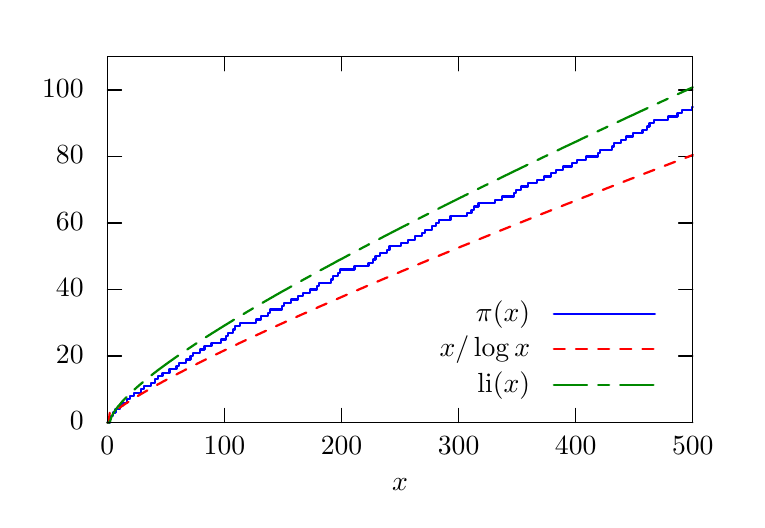
\begin{tikzpicture}[gnuplot]
%% generated with GNUPLOT 5.1p0 (Lua 5.3; terminal rev. 99, script rev. 100)
%% 木 11/22 15:28:55 2018
\path (0.000,0.000) rectangle (9.000,6.000);
\gpcolor{color=gp lt color border}
\gpsetlinetype{gp lt border}
\gpsetdashtype{gp dt solid}
\gpsetlinewidth{1.00}
\draw[gp path] (1.012,0.985)--(1.192,0.985);
\draw[gp path] (8.447,0.985)--(8.267,0.985);
\node[gp node right] at (0.828,0.985) {$0$};
\draw[gp path] (1.012,1.830)--(1.192,1.830);
\draw[gp path] (8.447,1.830)--(8.267,1.830);
\node[gp node right] at (0.828,1.830) {$20$};
\draw[gp path] (1.012,2.674)--(1.192,2.674);
\draw[gp path] (8.447,2.674)--(8.267,2.674);
\node[gp node right] at (0.828,2.674) {$40$};
\draw[gp path] (1.012,3.519)--(1.192,3.519);
\draw[gp path] (8.447,3.519)--(8.267,3.519);
\node[gp node right] at (0.828,3.519) {$60$};
\draw[gp path] (1.012,4.364)--(1.192,4.364);
\draw[gp path] (8.447,4.364)--(8.267,4.364);
\node[gp node right] at (0.828,4.364) {$80$};
\draw[gp path] (1.012,5.209)--(1.192,5.209);
\draw[gp path] (8.447,5.209)--(8.267,5.209);
\node[gp node right] at (0.828,5.209) {$100$};
\draw[gp path] (1.012,0.985)--(1.012,1.165);
\draw[gp path] (1.012,5.631)--(1.012,5.451);
\node[gp node center] at (1.012,0.677) {$0$};
\draw[gp path] (2.499,0.985)--(2.499,1.165);
\draw[gp path] (2.499,5.631)--(2.499,5.451);
\node[gp node center] at (2.499,0.677) {$100$};
\draw[gp path] (3.986,0.985)--(3.986,1.165);
\draw[gp path] (3.986,5.631)--(3.986,5.451);
\node[gp node center] at (3.986,0.677) {$200$};
\draw[gp path] (5.473,0.985)--(5.473,1.165);
\draw[gp path] (5.473,5.631)--(5.473,5.451);
\node[gp node center] at (5.473,0.677) {$300$};
\draw[gp path] (6.960,0.985)--(6.960,1.165);
\draw[gp path] (6.960,5.631)--(6.960,5.451);
\node[gp node center] at (6.960,0.677) {$400$};
\draw[gp path] (8.447,0.985)--(8.447,1.165);
\draw[gp path] (8.447,5.631)--(8.447,5.451);
\node[gp node center] at (8.447,0.677) {$500$};
\draw[gp path] (1.012,5.631)--(1.012,0.985)--(8.447,0.985)--(8.447,5.631)--cycle;
\node[gp node center] at (4.729,0.215) {$x$};
\node[gp node right] at (6.498,2.365) {$\pi(x)$};
\gpcolor{rgb color={0.000,0.000,1.000}}
\gpsetlinewidth{2.00}
\draw[gp path] (6.682,2.365)--(7.966,2.365);
\draw[gp path] (1.012,0.985)--(1.027,0.985)--(1.042,0.985)--(1.042,1.027)--(1.057,1.027)%
  --(1.057,1.069)--(1.071,1.069)--(1.086,1.069)--(1.086,1.112)--(1.101,1.112)--(1.116,1.112)%
  --(1.116,1.154)--(1.131,1.154)--(1.146,1.154)--(1.161,1.154)--(1.176,1.154)--(1.176,1.196)%
  --(1.190,1.196)--(1.205,1.196)--(1.205,1.238)--(1.220,1.238)--(1.235,1.238)--(1.250,1.238)%
  --(1.265,1.238)--(1.265,1.281)--(1.280,1.281)--(1.295,1.281)--(1.295,1.323)--(1.309,1.323)%
  --(1.324,1.323)--(1.339,1.323)--(1.354,1.323)--(1.354,1.365)--(1.369,1.365)--(1.384,1.365)%
  --(1.399,1.365)--(1.413,1.365)--(1.428,1.365)--(1.443,1.365)--(1.443,1.407)--(1.458,1.407)%
  --(1.473,1.407)--(1.473,1.450)--(1.488,1.450)--(1.503,1.450)--(1.518,1.450)--(1.532,1.450)%
  --(1.547,1.450)--(1.562,1.450)--(1.562,1.492)--(1.577,1.492)--(1.592,1.492)--(1.607,1.492)%
  --(1.622,1.492)--(1.622,1.534)--(1.637,1.534)--(1.651,1.534)--(1.651,1.576)--(1.666,1.576)%
  --(1.681,1.576)--(1.696,1.576)--(1.711,1.576)--(1.711,1.619)--(1.726,1.619)--(1.741,1.619)%
  --(1.756,1.619)--(1.770,1.619)--(1.785,1.619)--(1.800,1.619)--(1.800,1.661)--(1.815,1.661)%
  --(1.830,1.661)--(1.845,1.661)--(1.860,1.661)--(1.874,1.661)--(1.889,1.661)--(1.889,1.703)%
  --(1.904,1.703)--(1.919,1.703)--(1.919,1.745)--(1.934,1.745)--(1.949,1.745)--(1.964,1.745)%
  --(1.979,1.745)--(1.993,1.745)--(2.008,1.745)--(2.008,1.787)--(2.023,1.787)--(2.038,1.787)%
  --(2.053,1.787)--(2.068,1.787)--(2.068,1.830)--(2.083,1.830)--(2.098,1.830)--(2.098,1.872)%
  --(2.112,1.872)--(2.127,1.872)--(2.142,1.872)--(2.157,1.872)--(2.172,1.872)--(2.187,1.872)%
  --(2.187,1.914)--(2.202,1.914)--(2.216,1.914)--(2.231,1.914)--(2.246,1.914)--(2.246,1.956)%
  --(2.261,1.956)--(2.276,1.956)--(2.291,1.956)--(2.306,1.956)--(2.321,1.956)--(2.335,1.956)%
  --(2.335,1.999)--(2.350,1.999)--(2.365,1.999)--(2.380,1.999)--(2.395,1.999)--(2.410,1.999)%
  --(2.425,1.999)--(2.440,1.999)--(2.454,1.999)--(2.454,2.041)--(2.469,2.041)--(2.484,2.041)%
  --(2.499,2.041)--(2.514,2.041)--(2.514,2.083)--(2.529,2.083)--(2.544,2.083)--(2.544,2.125)%
  --(2.558,2.125)--(2.573,2.125)--(2.588,2.125)--(2.603,2.125)--(2.603,2.168)--(2.618,2.168)%
  --(2.633,2.168)--(2.633,2.210)--(2.648,2.210)--(2.663,2.210)--(2.677,2.210)--(2.692,2.210)%
  --(2.692,2.252)--(2.707,2.252)--(2.722,2.252)--(2.737,2.252)--(2.752,2.252)--(2.767,2.252)%
  --(2.782,2.252)--(2.796,2.252)--(2.811,2.252)--(2.826,2.252)--(2.841,2.252)--(2.856,2.252)%
  --(2.871,2.252)--(2.886,2.252)--(2.900,2.252)--(2.900,2.294)--(2.915,2.294)--(2.930,2.294)%
  --(2.945,2.294)--(2.960,2.294)--(2.960,2.337)--(2.975,2.337)--(2.990,2.337)--(3.005,2.337)%
  --(3.019,2.337)--(3.034,2.337)--(3.049,2.337)--(3.049,2.379)--(3.064,2.379)--(3.079,2.379)%
  --(3.079,2.421)--(3.094,2.421)--(3.109,2.421)--(3.124,2.421)--(3.138,2.421)--(3.153,2.421)%
  --(3.168,2.421)--(3.183,2.421)--(3.198,2.421)--(3.213,2.421)--(3.228,2.421)--(3.228,2.463)%
  --(3.243,2.463)--(3.257,2.463)--(3.257,2.506)--(3.272,2.506)--(3.287,2.506)--(3.302,2.506)%
  --(3.317,2.506)--(3.332,2.506)--(3.347,2.506)--(3.347,2.548)--(3.361,2.548)--(3.376,2.548)%
  --(3.391,2.548)--(3.406,2.548)--(3.421,2.548)--(3.436,2.548)--(3.436,2.590)--(3.451,2.590)%
  --(3.466,2.590)--(3.480,2.590)--(3.495,2.590)--(3.495,2.632)--(3.510,2.632)--(3.525,2.632)%
  --(3.540,2.632)--(3.555,2.632)--(3.570,2.632)--(3.585,2.632)--(3.585,2.674)--(3.599,2.674)%
  --(3.614,2.674)--(3.629,2.674)--(3.644,2.674)--(3.659,2.674)--(3.674,2.674)--(3.674,2.717)%
  --(3.689,2.717)--(3.703,2.717)--(3.703,2.759)--(3.718,2.759)--(3.733,2.759)--(3.748,2.759)%
  --(3.763,2.759)--(3.778,2.759)--(3.793,2.759)--(3.808,2.759)--(3.822,2.759)--(3.837,2.759)%
  --(3.852,2.759)--(3.852,2.801)--(3.867,2.801)--(3.882,2.801)--(3.882,2.843)--(3.897,2.843)%
  --(3.912,2.843)--(3.927,2.843)--(3.941,2.843)--(3.941,2.886)--(3.956,2.886)--(3.971,2.886)%
  --(3.971,2.928)--(3.986,2.928)--(4.001,2.928)--(4.016,2.928)--(4.031,2.928)--(4.045,2.928)%
  --(4.060,2.928)--(4.075,2.928)--(4.090,2.928)--(4.105,2.928)--(4.120,2.928)--(4.135,2.928)%
  --(4.150,2.928)--(4.150,2.970)--(4.164,2.970)--(4.179,2.970)--(4.194,2.970)--(4.209,2.970)%
  --(4.224,2.970)--(4.239,2.970)--(4.254,2.970)--(4.269,2.970)--(4.283,2.970)--(4.298,2.970)%
  --(4.313,2.970)--(4.328,2.970)--(4.328,3.012)--(4.343,3.012)--(4.358,3.012)--(4.373,3.012)%
  --(4.387,3.012)--(4.387,3.055)--(4.402,3.055)--(4.417,3.055)--(4.417,3.097)--(4.432,3.097)%
  --(4.447,3.097)--(4.462,3.097)--(4.477,3.097)--(4.477,3.139)--(4.492,3.139)--(4.506,3.139)%
  --(4.521,3.139)--(4.536,3.139)--(4.551,3.139)--(4.566,3.139)--(4.566,3.181)--(4.581,3.181)%
  --(4.596,3.181)--(4.596,3.224)--(4.611,3.224)--(4.625,3.224)--(4.640,3.224)--(4.655,3.224)%
  --(4.670,3.224)--(4.685,3.224)--(4.700,3.224)--(4.715,3.224)--(4.730,3.224)--(4.744,3.224)%
  --(4.744,3.266)--(4.759,3.266)--(4.774,3.266)--(4.789,3.266)--(4.804,3.266)--(4.819,3.266)%
  --(4.834,3.266)--(4.834,3.308)--(4.848,3.308)--(4.863,3.308)--(4.878,3.308)--(4.893,3.308)%
  --(4.908,3.308)--(4.923,3.308)--(4.923,3.350)--(4.938,3.350)--(4.953,3.350)--(4.967,3.350)%
  --(4.982,3.350)--(4.997,3.350)--(5.012,3.350)--(5.012,3.392)--(5.027,3.392)--(5.042,3.392)%
  --(5.042,3.435)--(5.057,3.435)--(5.072,3.435)--(5.086,3.435)--(5.101,3.435)--(5.116,3.435)%
  --(5.131,3.435)--(5.131,3.477)--(5.146,3.477)--(5.161,3.477)--(5.176,3.477)--(5.190,3.477)%
  --(5.190,3.519)--(5.205,3.519)--(5.220,3.519)--(5.220,3.561)--(5.235,3.561)--(5.250,3.561)%
  --(5.265,3.561)--(5.280,3.561)--(5.295,3.561)--(5.309,3.561)--(5.324,3.561)--(5.339,3.561)%
  --(5.354,3.561)--(5.369,3.561)--(5.369,3.604)--(5.384,3.604)--(5.399,3.604)--(5.414,3.604)%
  --(5.428,3.604)--(5.443,3.604)--(5.458,3.604)--(5.473,3.604)--(5.488,3.604)--(5.503,3.604)%
  --(5.518,3.604)--(5.532,3.604)--(5.547,3.604)--(5.562,3.604)--(5.577,3.604)--(5.577,3.646)%
  --(5.592,3.646)--(5.607,3.646)--(5.622,3.646)--(5.637,3.646)--(5.637,3.688)--(5.651,3.688)%
  --(5.666,3.688)--(5.666,3.730)--(5.681,3.730)--(5.696,3.730)--(5.711,3.730)--(5.726,3.730)%
  --(5.726,3.773)--(5.741,3.773)--(5.756,3.773)--(5.770,3.773)--(5.785,3.773)--(5.800,3.773)%
  --(5.815,3.773)--(5.830,3.773)--(5.845,3.773)--(5.860,3.773)--(5.874,3.773)--(5.889,3.773)%
  --(5.904,3.773)--(5.919,3.773)--(5.934,3.773)--(5.934,3.815)--(5.949,3.815)--(5.964,3.815)%
  --(5.979,3.815)--(5.993,3.815)--(6.008,3.815)--(6.023,3.815)--(6.023,3.857)--(6.038,3.857)%
  --(6.053,3.857)--(6.068,3.857)--(6.083,3.857)--(6.098,3.857)--(6.112,3.857)--(6.127,3.857)%
  --(6.142,3.857)--(6.157,3.857)--(6.172,3.857)--(6.172,3.899)--(6.187,3.899)--(6.202,3.899)%
  --(6.202,3.942)--(6.217,3.942)--(6.231,3.942)--(6.246,3.942)--(6.261,3.942)--(6.261,3.984)%
  --(6.276,3.984)--(6.291,3.984)--(6.306,3.984)--(6.321,3.984)--(6.335,3.984)--(6.350,3.984)%
  --(6.350,4.026)--(6.365,4.026)--(6.380,4.026)--(6.395,4.026)--(6.410,4.026)--(6.425,4.026)%
  --(6.440,4.026)--(6.454,4.026)--(6.469,4.026)--(6.469,4.068)--(6.484,4.068)--(6.499,4.068)%
  --(6.514,4.068)--(6.529,4.068)--(6.544,4.068)--(6.559,4.068)--(6.559,4.110)--(6.573,4.110)%
  --(6.588,4.110)--(6.603,4.110)--(6.618,4.110)--(6.633,4.110)--(6.648,4.110)--(6.648,4.153)%
  --(6.663,4.153)--(6.677,4.153)--(6.692,4.153)--(6.707,4.153)--(6.707,4.195)--(6.722,4.195)%
  --(6.737,4.195)--(6.752,4.195)--(6.767,4.195)--(6.782,4.195)--(6.796,4.195)--(6.796,4.237)%
  --(6.811,4.237)--(6.826,4.237)--(6.841,4.237)--(6.856,4.237)--(6.871,4.237)--(6.886,4.237)%
  --(6.901,4.237)--(6.915,4.237)--(6.915,4.279)--(6.930,4.279)--(6.945,4.279)--(6.960,4.279)%
  --(6.975,4.279)--(6.975,4.322)--(6.990,4.322)--(7.005,4.322)--(7.019,4.322)--(7.034,4.322)%
  --(7.049,4.322)--(7.064,4.322)--(7.079,4.322)--(7.094,4.322)--(7.094,4.364)--(7.109,4.364)%
  --(7.124,4.364)--(7.138,4.364)--(7.153,4.364)--(7.168,4.364)--(7.183,4.364)--(7.198,4.364)%
  --(7.213,4.364)--(7.228,4.364)--(7.243,4.364)--(7.243,4.406)--(7.257,4.406)--(7.272,4.406)%
  --(7.272,4.448)--(7.287,4.448)--(7.302,4.448)--(7.317,4.448)--(7.332,4.448)--(7.347,4.448)%
  --(7.361,4.448)--(7.376,4.448)--(7.391,4.448)--(7.406,4.448)--(7.421,4.448)--(7.421,4.491)%
  --(7.436,4.491)--(7.451,4.491)--(7.451,4.533)--(7.466,4.533)--(7.480,4.533)--(7.495,4.533)%
  --(7.510,4.533)--(7.525,4.533)--(7.540,4.533)--(7.540,4.575)--(7.555,4.575)--(7.570,4.575)%
  --(7.585,4.575)--(7.599,4.575)--(7.599,4.617)--(7.614,4.617)--(7.629,4.617)--(7.644,4.617)%
  --(7.659,4.617)--(7.674,4.617)--(7.689,4.617)--(7.689,4.660)--(7.704,4.660)--(7.718,4.660)%
  --(7.733,4.660)--(7.748,4.660)--(7.763,4.660)--(7.778,4.660)--(7.793,4.660)--(7.808,4.660)%
  --(7.808,4.702)--(7.822,4.702)--(7.837,4.702)--(7.852,4.702)--(7.867,4.702)--(7.867,4.744)%
  --(7.882,4.744)--(7.897,4.744)--(7.897,4.786)--(7.912,4.786)--(7.927,4.786)--(7.941,4.786)%
  --(7.956,4.786)--(7.956,4.829)--(7.971,4.829)--(7.986,4.829)--(8.001,4.829)--(8.016,4.829)%
  --(8.031,4.829)--(8.046,4.829)--(8.060,4.829)--(8.075,4.829)--(8.090,4.829)--(8.105,4.829)%
  --(8.120,4.829)--(8.135,4.829)--(8.135,4.871)--(8.150,4.871)--(8.164,4.871)--(8.179,4.871)%
  --(8.194,4.871)--(8.209,4.871)--(8.224,4.871)--(8.239,4.871)--(8.254,4.871)--(8.254,4.913)%
  --(8.269,4.913)--(8.283,4.913)--(8.298,4.913)--(8.313,4.913)--(8.313,4.955)--(8.328,4.955)%
  --(8.343,4.955)--(8.358,4.955)--(8.373,4.955)--(8.388,4.955)--(8.402,4.955)--(8.417,4.955)%
  --(8.432,4.955)--(8.432,4.997)--(8.447,4.997);
\gpcolor{color=gp lt color border}
\node[gp node right] at (6.498,1.915) {$x/\log x$};
\gpcolor{rgb color={1.000,0.000,0.000}}
\gpsetdashtype{dash pattern=on 5.00*\gpdashlength off 5.00*\gpdashlength }
\draw[gp path] (6.682,1.915)--(7.966,1.915);
\draw[gp path] (1.012,0.985)--(1.027,0.985)--(1.042,1.107)--(1.057,1.100)--(1.071,1.107)%
  --(1.086,1.116)--(1.101,1.126)--(1.116,1.137)--(1.131,1.147)--(1.146,1.158)--(1.161,1.168)%
  --(1.176,1.179)--(1.190,1.189)--(1.205,1.199)--(1.220,1.209)--(1.235,1.219)--(1.250,1.229)%
  --(1.265,1.238)--(1.280,1.248)--(1.295,1.258)--(1.309,1.267)--(1.324,1.276)--(1.339,1.286)%
  --(1.354,1.295)--(1.369,1.304)--(1.384,1.313)--(1.399,1.322)--(1.413,1.331)--(1.428,1.340)%
  --(1.443,1.349)--(1.458,1.358)--(1.473,1.366)--(1.488,1.375)--(1.503,1.384)--(1.518,1.392)%
  --(1.532,1.401)--(1.547,1.409)--(1.562,1.418)--(1.577,1.426)--(1.592,1.435)--(1.607,1.443)%
  --(1.622,1.451)--(1.637,1.460)--(1.651,1.468)--(1.666,1.476)--(1.681,1.484)--(1.696,1.492)%
  --(1.711,1.501)--(1.726,1.509)--(1.741,1.517)--(1.756,1.525)--(1.770,1.533)--(1.785,1.541)%
  --(1.800,1.549)--(1.815,1.557)--(1.830,1.565)--(1.845,1.573)--(1.860,1.580)--(1.874,1.588)%
  --(1.889,1.596)--(1.904,1.604)--(1.919,1.612)--(1.934,1.619)--(1.949,1.627)--(1.964,1.635)%
  --(1.979,1.643)--(1.993,1.650)--(2.008,1.658)--(2.023,1.666)--(2.038,1.673)--(2.053,1.681)%
  --(2.068,1.688)--(2.083,1.696)--(2.098,1.704)--(2.112,1.711)--(2.127,1.719)--(2.142,1.726)%
  --(2.157,1.734)--(2.172,1.741)--(2.187,1.749)--(2.202,1.756)--(2.216,1.764)--(2.231,1.771)%
  --(2.246,1.778)--(2.261,1.786)--(2.276,1.793)--(2.291,1.800)--(2.306,1.808)--(2.321,1.815)%
  --(2.335,1.822)--(2.350,1.830)--(2.365,1.837)--(2.380,1.844)--(2.395,1.852)--(2.410,1.859)%
  --(2.425,1.866)--(2.440,1.873)--(2.454,1.881)--(2.469,1.888)--(2.484,1.895)--(2.499,1.902)%
  --(2.514,1.909)--(2.529,1.916)--(2.544,1.924)--(2.558,1.931)--(2.573,1.938)--(2.588,1.945)%
  --(2.603,1.952)--(2.618,1.959)--(2.633,1.966)--(2.648,1.973)--(2.663,1.980)--(2.677,1.988)%
  --(2.692,1.995)--(2.707,2.002)--(2.722,2.009)--(2.737,2.016)--(2.752,2.023)--(2.767,2.030)%
  --(2.782,2.037)--(2.796,2.044)--(2.811,2.051)--(2.826,2.058)--(2.841,2.065)--(2.856,2.072)%
  --(2.871,2.078)--(2.886,2.085)--(2.900,2.092)--(2.915,2.099)--(2.930,2.106)--(2.945,2.113)%
  --(2.960,2.120)--(2.975,2.127)--(2.990,2.134)--(3.005,2.141)--(3.019,2.147)--(3.034,2.154)%
  --(3.049,2.161)--(3.064,2.168)--(3.079,2.175)--(3.094,2.182)--(3.109,2.188)--(3.124,2.195)%
  --(3.138,2.202)--(3.153,2.209)--(3.168,2.216)--(3.183,2.222)--(3.198,2.229)--(3.213,2.236)%
  --(3.228,2.243)--(3.243,2.249)--(3.257,2.256)--(3.272,2.263)--(3.287,2.270)--(3.302,2.276)%
  --(3.317,2.283)--(3.332,2.290)--(3.347,2.296)--(3.361,2.303)--(3.376,2.310)--(3.391,2.317)%
  --(3.406,2.323)--(3.421,2.330)--(3.436,2.337)--(3.451,2.343)--(3.466,2.350)--(3.480,2.357)%
  --(3.495,2.363)--(3.510,2.370)--(3.525,2.376)--(3.540,2.383)--(3.555,2.390)--(3.570,2.396)%
  --(3.585,2.403)--(3.599,2.410)--(3.614,2.416)--(3.629,2.423)--(3.644,2.429)--(3.659,2.436)%
  --(3.674,2.442)--(3.689,2.449)--(3.703,2.456)--(3.718,2.462)--(3.733,2.469)--(3.748,2.475)%
  --(3.763,2.482)--(3.778,2.488)--(3.793,2.495)--(3.808,2.501)--(3.822,2.508)--(3.837,2.514)%
  --(3.852,2.521)--(3.867,2.527)--(3.882,2.534)--(3.897,2.540)--(3.912,2.547)--(3.927,2.553)%
  --(3.941,2.560)--(3.956,2.566)--(3.971,2.573)--(3.986,2.579)--(4.001,2.586)--(4.016,2.592)%
  --(4.031,2.599)--(4.045,2.605)--(4.060,2.612)--(4.075,2.618)--(4.090,2.624)--(4.105,2.631)%
  --(4.120,2.637)--(4.135,2.644)--(4.150,2.650)--(4.164,2.657)--(4.179,2.663)--(4.194,2.669)%
  --(4.209,2.676)--(4.224,2.682)--(4.239,2.689)--(4.254,2.695)--(4.269,2.701)--(4.283,2.708)%
  --(4.298,2.714)--(4.313,2.721)--(4.328,2.727)--(4.343,2.733)--(4.358,2.740)--(4.373,2.746)%
  --(4.387,2.752)--(4.402,2.759)--(4.417,2.765)--(4.432,2.771)--(4.447,2.778)--(4.462,2.784)%
  --(4.477,2.790)--(4.492,2.797)--(4.506,2.803)--(4.521,2.809)--(4.536,2.816)--(4.551,2.822)%
  --(4.566,2.828)--(4.581,2.835)--(4.596,2.841)--(4.611,2.847)--(4.625,2.853)--(4.640,2.860)%
  --(4.655,2.866)--(4.670,2.872)--(4.685,2.879)--(4.700,2.885)--(4.715,2.891)--(4.730,2.897)%
  --(4.744,2.904)--(4.759,2.910)--(4.774,2.916)--(4.789,2.922)--(4.804,2.929)--(4.819,2.935)%
  --(4.834,2.941)--(4.848,2.947)--(4.863,2.954)--(4.878,2.960)--(4.893,2.966)--(4.908,2.972)%
  --(4.923,2.979)--(4.938,2.985)--(4.953,2.991)--(4.967,2.997)--(4.982,3.003)--(4.997,3.010)%
  --(5.012,3.016)--(5.027,3.022)--(5.042,3.028)--(5.057,3.034)--(5.072,3.041)--(5.086,3.047)%
  --(5.101,3.053)--(5.116,3.059)--(5.131,3.065)--(5.146,3.071)--(5.161,3.078)--(5.176,3.084)%
  --(5.190,3.090)--(5.205,3.096)--(5.220,3.102)--(5.235,3.108)--(5.250,3.115)--(5.265,3.121)%
  --(5.280,3.127)--(5.295,3.133)--(5.309,3.139)--(5.324,3.145)--(5.339,3.151)--(5.354,3.158)%
  --(5.369,3.164)--(5.384,3.170)--(5.399,3.176)--(5.414,3.182)--(5.428,3.188)--(5.443,3.194)%
  --(5.458,3.200)--(5.473,3.206)--(5.488,3.213)--(5.503,3.219)--(5.518,3.225)--(5.532,3.231)%
  --(5.547,3.237)--(5.562,3.243)--(5.577,3.249)--(5.592,3.255)--(5.607,3.261)--(5.622,3.267)%
  --(5.637,3.273)--(5.651,3.280)--(5.666,3.286)--(5.681,3.292)--(5.696,3.298)--(5.711,3.304)%
  --(5.726,3.310)--(5.741,3.316)--(5.756,3.322)--(5.770,3.328)--(5.785,3.334)--(5.800,3.340)%
  --(5.815,3.346)--(5.830,3.352)--(5.845,3.358)--(5.860,3.364)--(5.874,3.370)--(5.889,3.376)%
  --(5.904,3.382)--(5.919,3.388)--(5.934,3.395)--(5.949,3.401)--(5.964,3.407)--(5.979,3.413)%
  --(5.993,3.419)--(6.008,3.425)--(6.023,3.431)--(6.038,3.437)--(6.053,3.443)--(6.068,3.449)%
  --(6.083,3.455)--(6.098,3.461)--(6.112,3.467)--(6.127,3.473)--(6.142,3.479)--(6.157,3.485)%
  --(6.172,3.491)--(6.187,3.497)--(6.202,3.503)--(6.217,3.509)--(6.231,3.515)--(6.246,3.520)%
  --(6.261,3.526)--(6.276,3.532)--(6.291,3.538)--(6.306,3.544)--(6.321,3.550)--(6.335,3.556)%
  --(6.350,3.562)--(6.365,3.568)--(6.380,3.574)--(6.395,3.580)--(6.410,3.586)--(6.425,3.592)%
  --(6.440,3.598)--(6.454,3.604)--(6.469,3.610)--(6.484,3.616)--(6.499,3.622)--(6.514,3.628)%
  --(6.529,3.634)--(6.544,3.640)--(6.559,3.645)--(6.573,3.651)--(6.588,3.657)--(6.603,3.663)%
  --(6.618,3.669)--(6.633,3.675)--(6.648,3.681)--(6.663,3.687)--(6.677,3.693)--(6.692,3.699)%
  --(6.707,3.705)--(6.722,3.711)--(6.737,3.716)--(6.752,3.722)--(6.767,3.728)--(6.782,3.734)%
  --(6.796,3.740)--(6.811,3.746)--(6.826,3.752)--(6.841,3.758)--(6.856,3.764)--(6.871,3.769)%
  --(6.886,3.775)--(6.901,3.781)--(6.915,3.787)--(6.930,3.793)--(6.945,3.799)--(6.960,3.805)%
  --(6.975,3.811)--(6.990,3.817)--(7.005,3.822)--(7.019,3.828)--(7.034,3.834)--(7.049,3.840)%
  --(7.064,3.846)--(7.079,3.852)--(7.094,3.858)--(7.109,3.863)--(7.124,3.869)--(7.138,3.875)%
  --(7.153,3.881)--(7.168,3.887)--(7.183,3.893)--(7.198,3.898)--(7.213,3.904)--(7.228,3.910)%
  --(7.243,3.916)--(7.257,3.922)--(7.272,3.928)--(7.287,3.934)--(7.302,3.939)--(7.317,3.945)%
  --(7.332,3.951)--(7.347,3.957)--(7.361,3.963)--(7.376,3.968)--(7.391,3.974)--(7.406,3.980)%
  --(7.421,3.986)--(7.436,3.992)--(7.451,3.998)--(7.466,4.003)--(7.480,4.009)--(7.495,4.015)%
  --(7.510,4.021)--(7.525,4.027)--(7.540,4.032)--(7.555,4.038)--(7.570,4.044)--(7.585,4.050)%
  --(7.599,4.056)--(7.614,4.061)--(7.629,4.067)--(7.644,4.073)--(7.659,4.079)--(7.674,4.085)%
  --(7.689,4.090)--(7.704,4.096)--(7.718,4.102)--(7.733,4.108)--(7.748,4.113)--(7.763,4.119)%
  --(7.778,4.125)--(7.793,4.131)--(7.808,4.137)--(7.822,4.142)--(7.837,4.148)--(7.852,4.154)%
  --(7.867,4.160)--(7.882,4.165)--(7.897,4.171)--(7.912,4.177)--(7.927,4.183)--(7.941,4.188)%
  --(7.956,4.194)--(7.971,4.200)--(7.986,4.206)--(8.001,4.211)--(8.016,4.217)--(8.031,4.223)%
  --(8.046,4.229)--(8.060,4.234)--(8.075,4.240)--(8.090,4.246)--(8.105,4.252)--(8.120,4.257)%
  --(8.135,4.263)--(8.150,4.269)--(8.164,4.275)--(8.179,4.280)--(8.194,4.286)--(8.209,4.292)%
  --(8.224,4.297)--(8.239,4.303)--(8.254,4.309)--(8.269,4.315)--(8.283,4.320)--(8.298,4.326)%
  --(8.313,4.332)--(8.328,4.337)--(8.343,4.343)--(8.358,4.349)--(8.373,4.355)--(8.388,4.360)%
  --(8.402,4.366)--(8.417,4.372)--(8.432,4.377)--(8.447,4.383);
\gpcolor{color=gp lt color border}
\node[gp node right] at (6.498,1.465) {$\mathrm{li}(x)$};
\gpcolor{rgb color={0.000,0.533,0.000}}
\gpsetdashtype{dash pattern=on 15.00*\gpdashlength off 5.00*\gpdashlength on 5.00*\gpdashlength off 5.00*\gpdashlength }
\draw[gp path] (6.682,1.465)--(7.966,1.465);
\draw[gp path] (1.012,0.985)--(1.027,0.985)--(1.042,0.985)--(1.057,1.037)--(1.071,1.071)%
  --(1.086,1.099)--(1.101,1.123)--(1.116,1.146)--(1.131,1.167)--(1.146,1.187)--(1.161,1.203)%
  --(1.176,1.221)--(1.190,1.239)--(1.205,1.256)--(1.220,1.272)--(1.235,1.288)--(1.250,1.303)%
  --(1.265,1.318)--(1.280,1.333)--(1.295,1.347)--(1.309,1.362)--(1.324,1.376)--(1.339,1.389)%
  --(1.354,1.403)--(1.369,1.416)--(1.384,1.430)--(1.399,1.443)--(1.413,1.455)--(1.428,1.468)%
  --(1.443,1.481)--(1.458,1.493)--(1.473,1.506)--(1.488,1.518)--(1.503,1.530)--(1.518,1.542)%
  --(1.532,1.554)--(1.547,1.566)--(1.562,1.578)--(1.577,1.590)--(1.592,1.602)--(1.607,1.614)%
  --(1.622,1.625)--(1.637,1.636)--(1.651,1.648)--(1.666,1.659)--(1.681,1.670)--(1.696,1.681)%
  --(1.711,1.692)--(1.726,1.703)--(1.741,1.714)--(1.756,1.725)--(1.770,1.735)--(1.785,1.746)%
  --(1.800,1.757)--(1.815,1.767)--(1.830,1.778)--(1.845,1.788)--(1.860,1.799)--(1.874,1.809)%
  --(1.889,1.820)--(1.904,1.830)--(1.919,1.840)--(1.934,1.851)--(1.949,1.861)--(1.964,1.871)%
  --(1.979,1.881)--(1.993,1.891)--(2.008,1.901)--(2.023,1.911)--(2.038,1.921)--(2.053,1.931)%
  --(2.068,1.941)--(2.083,1.951)--(2.098,1.961)--(2.112,1.971)--(2.127,1.980)--(2.142,1.990)%
  --(2.157,2.000)--(2.172,2.010)--(2.187,2.019)--(2.202,2.029)--(2.216,2.039)--(2.231,2.048)%
  --(2.246,2.058)--(2.261,2.067)--(2.276,2.077)--(2.291,2.086)--(2.306,2.096)--(2.321,2.105)%
  --(2.335,2.115)--(2.350,2.124)--(2.365,2.133)--(2.380,2.143)--(2.395,2.152)--(2.410,2.161)%
  --(2.425,2.171)--(2.440,2.180)--(2.454,2.189)--(2.469,2.198)--(2.484,2.208)--(2.499,2.217)%
  --(2.514,2.226)--(2.529,2.235)--(2.544,2.244)--(2.558,2.253)--(2.573,2.262)--(2.588,2.271)%
  --(2.603,2.281)--(2.618,2.290)--(2.633,2.299)--(2.648,2.308)--(2.663,2.317)--(2.677,2.326)%
  --(2.692,2.334)--(2.707,2.343)--(2.722,2.352)--(2.737,2.361)--(2.752,2.370)--(2.767,2.379)%
  --(2.782,2.388)--(2.796,2.397)--(2.811,2.405)--(2.826,2.414)--(2.841,2.423)--(2.856,2.432)%
  --(2.871,2.441)--(2.886,2.449)--(2.900,2.458)--(2.915,2.467)--(2.930,2.475)--(2.945,2.484)%
  --(2.960,2.493)--(2.975,2.501)--(2.990,2.510)--(3.005,2.519)--(3.019,2.527)--(3.034,2.536)%
  --(3.049,2.544)--(3.064,2.553)--(3.079,2.562)--(3.094,2.570)--(3.109,2.579)--(3.124,2.587)%
  --(3.138,2.596)--(3.153,2.604)--(3.168,2.613)--(3.183,2.621)--(3.198,2.630)--(3.213,2.638)%
  --(3.228,2.647)--(3.243,2.655)--(3.257,2.663)--(3.272,2.671)--(3.287,2.679)--(3.302,2.688)%
  --(3.317,2.696)--(3.332,2.705)--(3.347,2.713)--(3.361,2.721)--(3.376,2.730)--(3.391,2.738)%
  --(3.406,2.746)--(3.421,2.755)--(3.436,2.763)--(3.451,2.771)--(3.466,2.779)--(3.480,2.788)%
  --(3.495,2.796)--(3.510,2.804)--(3.525,2.812)--(3.540,2.821)--(3.555,2.829)--(3.570,2.837)%
  --(3.585,2.845)--(3.599,2.853)--(3.614,2.862)--(3.629,2.870)--(3.644,2.878)--(3.659,2.886)%
  --(3.674,2.894)--(3.689,2.902)--(3.703,2.911)--(3.718,2.919)--(3.733,2.927)--(3.748,2.935)%
  --(3.763,2.943)--(3.778,2.951)--(3.793,2.959)--(3.808,2.967)--(3.822,2.975)--(3.837,2.983)%
  --(3.852,2.991)--(3.867,2.999)--(3.882,3.007)--(3.897,3.016)--(3.912,3.024)--(3.927,3.032)%
  --(3.941,3.040)--(3.956,3.048)--(3.971,3.056)--(3.986,3.063)--(4.001,3.071)--(4.016,3.079)%
  --(4.031,3.087)--(4.045,3.095)--(4.060,3.103)--(4.075,3.111)--(4.090,3.119)--(4.105,3.127)%
  --(4.120,3.135)--(4.135,3.143)--(4.150,3.151)--(4.164,3.159)--(4.179,3.166)--(4.194,3.174)%
  --(4.209,3.182)--(4.224,3.190)--(4.239,3.198)--(4.254,3.206)--(4.269,3.214)--(4.283,3.221)%
  --(4.298,3.229)--(4.313,3.237)--(4.328,3.245)--(4.343,3.253)--(4.358,3.261)--(4.373,3.268)%
  --(4.387,3.276)--(4.402,3.284)--(4.417,3.292)--(4.432,3.299)--(4.447,3.307)--(4.462,3.315)%
  --(4.477,3.323)--(4.492,3.330)--(4.506,3.338)--(4.521,3.346)--(4.536,3.354)--(4.551,3.361)%
  --(4.566,3.369)--(4.581,3.377)--(4.596,3.385)--(4.611,3.392)--(4.625,3.400)--(4.640,3.408)%
  --(4.655,3.415)--(4.670,3.423)--(4.685,3.431)--(4.700,3.438)--(4.715,3.446)--(4.730,3.454)%
  --(4.744,3.461)--(4.759,3.469)--(4.774,3.477)--(4.789,3.484)--(4.804,3.492)--(4.819,3.499)%
  --(4.834,3.507)--(4.848,3.515)--(4.863,3.522)--(4.878,3.530)--(4.893,3.537)--(4.908,3.545)%
  --(4.923,3.553)--(4.938,3.560)--(4.953,3.568)--(4.967,3.575)--(4.982,3.583)--(4.997,3.590)%
  --(5.012,3.598)--(5.027,3.606)--(5.042,3.613)--(5.057,3.621)--(5.072,3.628)--(5.086,3.636)%
  --(5.101,3.643)--(5.116,3.651)--(5.131,3.658)--(5.146,3.666)--(5.161,3.673)--(5.176,3.681)%
  --(5.190,3.688)--(5.205,3.696)--(5.220,3.703)--(5.235,3.711)--(5.250,3.718)--(5.265,3.726)%
  --(5.280,3.733)--(5.295,3.741)--(5.309,3.748)--(5.324,3.755)--(5.339,3.763)--(5.354,3.770)%
  --(5.369,3.778)--(5.384,3.785)--(5.399,3.793)--(5.414,3.800)--(5.428,3.807)--(5.443,3.815)%
  --(5.458,3.822)--(5.473,3.830)--(5.488,3.837)--(5.503,3.845)--(5.518,3.852)--(5.532,3.859)%
  --(5.547,3.867)--(5.562,3.874)--(5.577,3.881)--(5.592,3.889)--(5.607,3.896)--(5.622,3.904)%
  --(5.637,3.911)--(5.651,3.918)--(5.666,3.926)--(5.681,3.933)--(5.696,3.940)--(5.711,3.948)%
  --(5.726,3.955)--(5.741,3.962)--(5.756,3.970)--(5.770,3.977)--(5.785,3.984)--(5.800,3.992)%
  --(5.815,3.999)--(5.830,4.006)--(5.845,4.014)--(5.860,4.021)--(5.874,4.028)--(5.889,4.035)%
  --(5.904,4.043)--(5.919,4.050)--(5.934,4.057)--(5.949,4.065)--(5.964,4.072)--(5.979,4.079)%
  --(5.993,4.086)--(6.008,4.094)--(6.023,4.101)--(6.038,4.108)--(6.053,4.115)--(6.068,4.123)%
  --(6.083,4.130)--(6.098,4.137)--(6.112,4.144)--(6.127,4.152)--(6.142,4.159)--(6.157,4.166)%
  --(6.172,4.173)--(6.187,4.181)--(6.202,4.188)--(6.217,4.195)--(6.231,4.202)--(6.246,4.209)%
  --(6.261,4.217)--(6.276,4.224)--(6.291,4.231)--(6.306,4.238)--(6.321,4.245)--(6.335,4.253)%
  --(6.350,4.260)--(6.365,4.267)--(6.380,4.274)--(6.395,4.281)--(6.410,4.288)--(6.425,4.296)%
  --(6.440,4.303)--(6.454,4.310)--(6.469,4.317)--(6.484,4.324)--(6.499,4.331)--(6.514,4.338)%
  --(6.529,4.346)--(6.544,4.353)--(6.559,4.360)--(6.573,4.367)--(6.588,4.374)--(6.603,4.381)%
  --(6.618,4.388)--(6.633,4.396)--(6.648,4.403)--(6.663,4.410)--(6.677,4.417)--(6.692,4.424)%
  --(6.707,4.431)--(6.722,4.438)--(6.737,4.445)--(6.752,4.452)--(6.767,4.459)--(6.782,4.467)%
  --(6.796,4.474)--(6.811,4.481)--(6.826,4.488)--(6.841,4.495)--(6.856,4.502)--(6.871,4.509)%
  --(6.886,4.516)--(6.901,4.523)--(6.915,4.530)--(6.930,4.537)--(6.945,4.544)--(6.960,4.551)%
  --(6.975,4.558)--(6.990,4.565)--(7.005,4.572)--(7.019,4.579)--(7.034,4.587)--(7.049,4.594)%
  --(7.064,4.601)--(7.079,4.608)--(7.094,4.615)--(7.109,4.622)--(7.124,4.629)--(7.138,4.636)%
  --(7.153,4.643)--(7.168,4.650)--(7.183,4.657)--(7.198,4.664)--(7.213,4.671)--(7.228,4.678)%
  --(7.243,4.685)--(7.257,4.692)--(7.272,4.699)--(7.287,4.706)--(7.302,4.713)--(7.317,4.720)%
  --(7.332,4.727)--(7.347,4.734)--(7.361,4.741)--(7.376,4.748)--(7.391,4.755)--(7.406,4.762)%
  --(7.421,4.768)--(7.436,4.775)--(7.451,4.782)--(7.466,4.789)--(7.480,4.796)--(7.495,4.803)%
  --(7.510,4.810)--(7.525,4.817)--(7.540,4.824)--(7.555,4.831)--(7.570,4.838)--(7.585,4.845)%
  --(7.599,4.852)--(7.614,4.859)--(7.629,4.866)--(7.644,4.873)--(7.659,4.880)--(7.674,4.886)%
  --(7.689,4.893)--(7.704,4.900)--(7.718,4.907)--(7.733,4.914)--(7.748,4.921)--(7.763,4.928)%
  --(7.778,4.935)--(7.793,4.942)--(7.808,4.949)--(7.822,4.956)--(7.837,4.962)--(7.852,4.969)%
  --(7.867,4.976)--(7.882,4.983)--(7.897,4.990)--(7.912,4.997)--(7.927,5.004)--(7.941,5.011)%
  --(7.956,5.017)--(7.971,5.024)--(7.986,5.031)--(8.001,5.038)--(8.016,5.045)--(8.031,5.052)%
  --(8.046,5.059)--(8.060,5.066)--(8.075,5.072)--(8.090,5.079)--(8.105,5.086)--(8.120,5.093)%
  --(8.135,5.100)--(8.150,5.107)--(8.164,5.113)--(8.179,5.120)--(8.194,5.127)--(8.209,5.134)%
  --(8.224,5.141)--(8.239,5.148)--(8.254,5.154)--(8.269,5.161)--(8.283,5.168)--(8.298,5.175)%
  --(8.313,5.182)--(8.328,5.189)--(8.343,5.195)--(8.358,5.202)--(8.373,5.209)--(8.388,5.216)%
  --(8.402,5.223)--(8.417,5.229)--(8.432,5.236)--(8.447,5.243);
\gpcolor{color=gp lt color border}
\gpsetdashtype{gp dt solid}
\gpsetlinewidth{1.00}
\draw[gp path] (1.012,5.631)--(1.012,0.985)--(8.447,0.985)--(8.447,5.631)--cycle;
%% coordinates of the plot area
\gpdefrectangularnode{gp plot 1}{\pgfpoint{1.012cm}{0.985cm}}{\pgfpoint{8.447cm}{5.631cm}}
\end{tikzpicture}

%   \caption{$\pi(x)$とその近似式}
%   % \label{fig:00}
% \end{figure}

\end{document}